\documentclass[serif,xcolor=pdftex,dvipsnames,table,hyperref={bookmarks=false,breaklinks}]{beamer}

%%%%%%%%%%%%%%%%
% Change the macros below to configure the title slides
% for your course.
\newcommand{\coursename}{COMPSCI 589}
\newcommand{\instructor}{Benjamin M. Marlin}
\newcommand{\university}{University of Massachusetts Amherst}
\newcommand{\department}{College of Information and Computer Sciences}
%%%%%%%%%%%%%%%%


\newcommand{\settitlecard}[2]{
  \title[\coursename  Lecture #1] 
    {\coursename \\ Lecture #1: #2}
     \author[\instructor]{\instructor}
     \institute[\university]{
     \department\\
     \university
   }
\date{}
}

\newcommand{\maketitlepage}{
  \begin{frame}
  \titlepage
  \center{
    %If you use the slides unmodified, retain the attribution below
    \tiny{Slides by Benjamin M. Marlin (marlin@cs.umass.edu). \\
    \vspace{-1em}Created with support from National Science Foundation Award\# IIS-1350522. 
    %If you modify the slides, please retain the alternate attribution below
    %\tiny{Based on slides by Benjamin M. Marlin (marlin@cs.umass.edu). \\    
    %\vspace{-1em}Created with support from National Science Foundation Award\# IIS-1350522. 
    }                                              
  }  
  \end{frame}
}

\AtBeginSection[]
{
  \begin{frame}<beamer>{Outline}
    \tableofcontents[currentsection,subsectionstyle=hide]
  \end{frame}
}


\newcommand{\cut}[1]{}

\newcommand{\iconbox}[4]{
  \only<#1-#2>{
    \begin{columns}[T]
      \column{0.5in}
           \includegraphics[width=0.5in]{#3}
       \column{3.7in}
            #4
    \end{columns}
    \medskip
    \medskip
    \medskip
  }
}

\mode<presentation>{
  \usepackage{../beamertheme589theme}
  \setbeamercovered{invisible}
}

\mode<handout>{
  \usepackage{../beamertheme589theme}
  \setbeamercovered{transparent}
}


\usepackage[english]{babel}
\usepackage[latin1]{inputenc}
\usepackage{times}
\usepackage[T1]{fontenc}
\usepackage{amsmath}
\usepackage{amssymb}
\usepackage[noend]{algorithmic}
\usepackage{algorithm}
\usepackage{listings}

\renewcommand\mathfamilydefault{\rmdefault}

\newcommand{\setA}{\mathcal{A}}
\newcommand{\setB}{\mathcal{B}}
\newcommand{\setS}{\mathcal{S}}
\newcommand{\setV}{\mathcal{V}}
\DeclareMathOperator*{\union}{\bigcup}
\DeclareMathOperator*{\intersection}{\bigcap}
\DeclareMathOperator*{\Val}{Val}
\newcommand{\mbf}[1]{{\mathbf{#1}}}
\DeclareMathOperator*{\argmax}{arg\,max}
\DeclareMathOperator*{\argmin}{arg\,min}
\DeclareMathOperator*{\sign}{sign}
\newcommand{\deriv}[2]{\frac{\partial{#1}}{\partial{#2}}}


\settitlecard{22}{Multidimensional Scaling and Isomap}

\begin{document}

\maketitlepage


\section{Review}
\subsection{Foo}

\begin{frame}[t]{Kernel PCA and Spectral Clustering}

\begin{itemize}
\item Last class, we saw a method to achieve non-linear dimensionality reduction
by combining basis expansions with dimensionality reduction.

\pause\item We showed that basis expansion can be combined with PCA and SVD, but that
PCA could also be used with the kernel trick.

\pause\item Lastly, we saw how spectral clustering can be viewed as a modification of 
clustering in the kernel PCA latent space.

\end{itemize} 
\end{frame}


\section{MDS}
\subsection{foo}


\begin{frame}[t]{Multidimensional Scaling}

\begin{itemize}
\item MDS is a non-linear dimensionality reduction method that is explicitly 
designed to minimize the distortion in the pairwise distances 
between points when projecting them into a low dimensional embedding.

\pause\item Suppose we have a data set $\mathcal{D}= 
\{\mbf{x}_i\in\mathbb{R}^D\}_{i=1:N}$. 

\pause\item Let $d_{ij}$ be the distance between $\mbf{x}_i$ and $\mbf{x}_j$. 
Any distance metric can be used. Euclidean distance  
$d_{ij}=||\mbf{x}_i-\mbf{x}_j||$ is common.

\end{itemize} 
\end{frame}

\begin{frame}[t]{Least Squares Multidimensional Scaling}

\begin{itemize}
\item Let $\mbf{z}_i \in \mathbb{R}^{K}$ be the low-dimensional embedding of 
$\mbf{x}_i$ for each data case $i$. We assume $K<D$.

\pause\item Least-squares MDS learns the embeddings $\mbf{z}_i$ by minimizing 
the following objective function, known as the \textit{stress} function:

\pause

$$\min_{\mathbf{z}_1,...,\mathbf{z}_N} \sum_{i<j} \left( d_{ij} - 
||\mbf{z}_i-\mbf{z}_j||_2\right)^2$$

\pause\item Basically, this function attempts to have the regular Euclidean 
distances between points in $\mathbb{R}^K$ reflect the distances between the 
points in $\mathbb{R}^D$. This can be useful for data visualization when $K=2$.

\end{itemize} 
\end{frame}

\begin{frame}[t]{Classical Multidimensional Scaling Variants}

\begin{itemize}
\item Let $s_{ij}$ be the similarity between $\mbf{x}_i$ and $\mbf{x}_j$. 


\pause\item Let $\mbf{z}_i \in \mathbb{R}^{K}$ be the low-dimensional embedding 
of $\mbf{x}_i$ for each data case $i$. We assume $K<D$.

\pause\item Classical MDS learns the embeddings $\mbf{z}_i$ by minimizing 
the following objective function:

\pause

$$\min_{\mathbf{z}_1,...,\mathbf{z}_N} \sum_{i<j} \left( s_{ij} - 
\langle \mbf{z}_i-\bar{\mbf{z}}, \mbf{z}_j-\bar{\mbf{z}}\rangle \right)^2$$

\pause\item If the similarities are centered inner products in $\mathbb{R}^D$, 
Classical MDS and PCA are equivalent. For other similarity functions, classical 
MDS performs non-linear dimensionality reduction.

\end{itemize}  
\end{frame}

\begin{frame}[t]{MDS Trade-offs}

\begin{itemize}
\item Interestingly, to use MDS we actually don't need the raw feature vectors. 
It's enough to have the pairwise distance or similarity matrices.

\pause\item Unlike kernel PCA, the similarity or distance matrices do not need 
to be valid kernel matrices (ie: they do not need to correspond to inner 
products of some basis expansion).

\pause\item A significant issue with MDS is that we need to be able to specify 
a global similarity or distance matrix directly. This may not actually be easy 
to do if the data come from a complex manifold (regular Euclidean distance will 
fail).

\end{itemize}  
\end{frame}



\section{Isomap}
\subsection{foo}


\begin{frame}[t]{Isometric feature mapping}

\begin{itemize}
\item Isometric feature mapping (Isomap) is a non-linear dimensionality 
reduction method that is designed to minimize the distortion in geodesic 
distances on a manifold when projecting them into a low dimensional embedding.
\end{itemize} 

\pause
\center
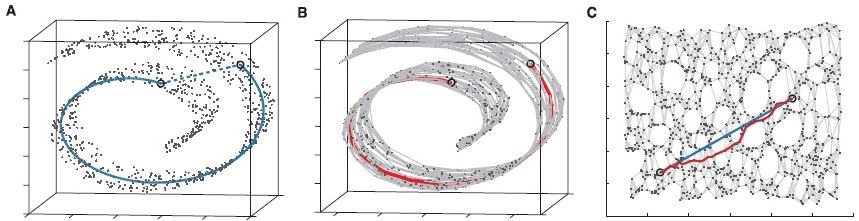
\includegraphics[width=4.5in]{../Figures/isomap.jpg}


\end{frame}

\begin{frame}[t]{Isometric feature mapping algorithm}
\begin{itemize}

\item The isomap algorithm begins by computing the K-nearest 
neighbors of each data point and building the distance weighted K-nearest 
neighbor graph $G$ over the data. 

\pause\item For points $i, j$ that are neighbors in the graph, isomap uses the 
straight line distance between them as $d_{ij}$.

\pause\item For points $i, j$ that are not neighbors in the graph, isomap uses 
the length of the shortest path in $G$ as $d_{ij}$. This is an approximation to
the geodesic distance between $\mbf{x}_i$ and $\mbf{x}_j$ on the manifold.

\pause\item Finally, isomap plugs the distances $d_{ij}$ into MDS with 
classical scaling and computes the embedding.

\end{itemize} 
\end{frame}



\end{document}
